\documentclass{beamer}
\usepackage[utf8]{inputenc}
\usetheme{Warsaw}
\usepackage{url}
\usepackage{verbatim}
\usepackage[french]{babel}
% permet d'avoir les numéros de pages:
\expandafter\def\expandafter\insertshorttitle\expandafter{%
    \insertshorttitle\hfill%
        \insertframenumber\,/\,\inserttotalframenumber}
% permet de voir où on en est entre chaque (sub)sections
\AtBeginSubsection[] {
    \begin{frame}<beamer>{Plan}
        \tableofcontents[currentsection, currentsubsection]
    \end{frame}
}
\begin{document}

%%%%%%%%%%%%%%%%%%%%%%%%%%%%%%%%%%%%%%%%%%%%%%%%%%%%%%%%%%%%%%%%%%%%%%%%%%%%%%%%%%%%%%%%%%%%%%%%
\title{Accès structurés \& interopérabilité}
\author{Yoann Ricordel, \\João Prado, \\Cédric Honnet}
\institute{Télécom ParisTech\\Robotique \& Systèmes Embarqués}
\titlepage

%%%%%%%%%%%%%%%%%%%%%%%%%%%%%%%%%%%%%%%%%%%%%%%%%%%%%%%%%%%%%%%%%%%%%%%%%%%%%%%%%%%%%%%%%%%%%%%%
\section{Plan}
    \begin{frame}
        \frametitle{Plan}
        \tableofcontents
    \end{frame}

%%%%%%%%%%%%%%%%%%%%%%%%%%%%%%%%%%%%%%%%%%%%%%%%%%%%%%%%%%%%%%%%%%%%%%%%%%%%%%%%%%%%%%%%%%%%%%%%
\section{Accès structurés}

    \subsection{REST}
        \begin{frame}
            \frametitle{REpresentational State Transfer}
            \begin{itemize}
                \item REST n'est ni un protocole, ni un standard \pause
                \item Style d’architecture pour systèmes d'information distribués \pause
                \item Elaboré en 2000 par Roy Fielding, un des créateurs du protocole HTTP
            \end{itemize}
        \end{frame}

        \begin{frame}
            \frametitle{Concept}
            \begin{itemize}
                \item Exemple avec HTTP : 
                \begin{center}
                    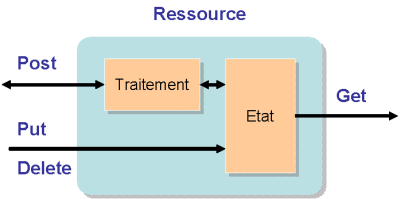
\includegraphics[width=0.5\textwidth]{get-post} \\
                    \tiny Source: figer.com 
                \end{center}
                \item Une ``ressource'' est une chose nommable (ex : site web)
                \item Une ``représentation'' est une séquence d’octets (ex : image)
                \item Un ``composant'' est un acteur, relié à d’autres composants/ressources par des canaux (ex : serveur)
            \end{itemize}
        \end{frame}

        \begin{frame}
            \frametitle{Contraintes}
            Définition :
            \begin{itemize}
                \item Client–server 
                \item Stateless (pas chez le client)
                \item Uniform interface (URI)
                \item Cacheable (évite une requête inutile)
                \item Layered system (ressources distribuées)
            \end{itemize}
            \pause
            Permettent d'optimiser :
            \begin{itemize}
                \item la simplicité
                \item la généricité
                \item les performances réseaux 
            \end{itemize}
        \end{frame}

%%%%%%%%%%%%%%%%%%%%%%%%%%%%%%%%%%%%%%%%%%%%%%%%%%%%%%%%%%%%%%%%%%%%%%%%%%%%%%%%%%%%%%%%%%%%%%%%
\subsection{CoAP}
\begin{frame}
  \frametitle{REST et l'embarqué}
  \begin{itemize}
  \item Protocoles de l'Internet classique : pas forcément adaptés à
    l'embarqué
  \item Contraintes de mémoire, puissance de calcul, consommation,
    environnementales, etc.
  \item Exemple : réseau de capteurs sans fil
    \pause   
  \item Pourtant, l'architecture REST reste souhaitable
    \pause
  \item Groupe de travail CoRE (Constrained RESTful Environments),
    de l'IETF (Internet Engineering Task Force)
  \end{itemize}
\end{frame}

\begin{frame}
  \frametitle{CoAP~: Constrained Application Protocol}
  \begin{itemize}
  \item Protocole web adapté pour les réseaux contraints
    \pause
  \item But~: implémenter un sous-ensemble de REST avec des
    optimisations pour les réseaux contraints
    \pause
  \item Correspondance avec HTTP
    \pause
  \item Basé sur UDP : messages asynchrones
    \pause
  \item Basse complexité + entêtes compactes
    \pause
  \item Fonctionnalités supplémentaires : proxy, cache, multicast, découverte de
    ressources...
  \end{itemize}
\end{frame}

\begin{frame}
  \frametitle{Format des messages}
  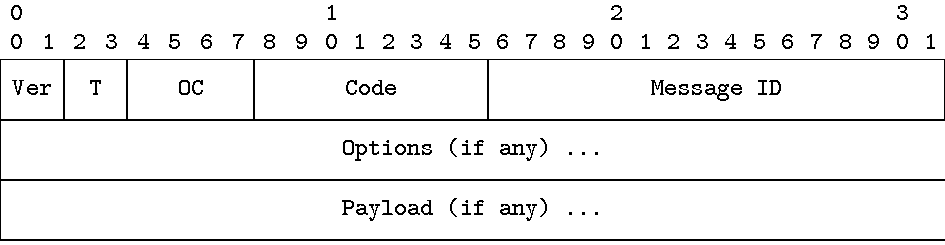
\includegraphics[width=\textwidth]{coap_packet}
  \begin{center}
    \tiny Source : draft-ietf-core-coap-04
  \end{center}
  \begin{itemize}
  \item \texttt{Ver} : version
  \item \texttt{T} : type
    \begin{itemize}
    \item Confirmable (\texttt{CON})
    \item Non-Confirmable (\texttt{NON})
    \item Acknowledgement (\texttt{ACK})
    \item Reset (\texttt{RST})
    \end{itemize}
  \item \texttt{OC} : Option Count
  \end{itemize}
\end{frame}

\begin{frame}
  \frametitle{Exemple (1/2)}
  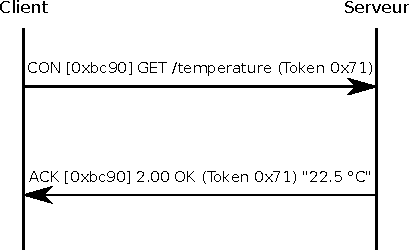
\includegraphics[width=\textwidth]{ex1}
  \begin{center}
    \tiny Source : draft-ietf-core-coap-04
  \end{center}
\end{frame}

\begin{frame}
  \frametitle{Exemple (2/2)}
  \begin{center}
  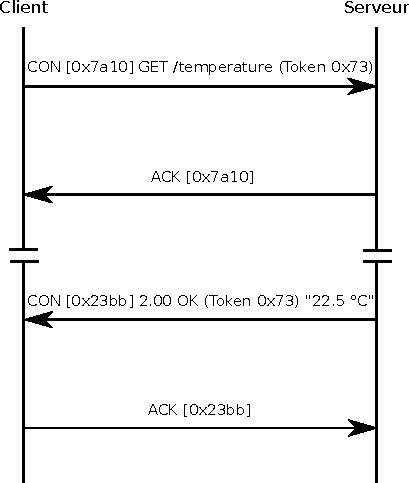
\includegraphics[height=0.8\textheight]{ex2}\\
    \tiny Source : draft-ietf-core-coap-04
  \end{center}
\end{frame}

%%%%%%%%%%%%%%%%%%%%%%%%%%%%%%%%%%%%%%%%%%%%%%%%%%%%%%%%%%%%%%%%%%%%%%%%%%%%%%%%%%%%%%%%%%%%%%%%
\section{Interopérabilité}

    \subsection{Problématique}
        \begin{frame}
            \frametitle{Problématique}
            \begin{itemize}
                \item Maintenant qu'on sait comment échanger des informations, il faudrait les représenter \pause
                \item Il est peu utile d'avoir des protocoles normalisés si la manière de coder les informations est propre à chacun \pause
                \item \textbf{Solution :} normaliser aussi les formats d'échange de données \pause
                        \begin{itemize}
                            \item XML
                            \item JSON
                        \end{itemize}
                
            \end{itemize}
        \end{frame}
    

    \subsection{XML}
        \begin{frame}[containsverbatim]
            \frametitle{XML : eXtensible Markup Language}
            \begin{itemize}
                \item \normalsize Basé sur des balises contenant éventuellement des attributs
                \footnotesize
                \begin{verbatim}    <balise attribut="attribut">Contenu de la balise</balise> \end{verbatim}
                \item \normalsize Permet la structuration hiérarchique d'information :
                \footnotesize
                \begin{verbatim}
    <article author="Jean Dupont">
        <titre>Titre de l'article </article>
        <sommaire>
            <article id="1" title="Introduction" />
            ...
        </sommaire>
        <contenu>
            <chapitre>...</chapitre>
        </contenu>
    </article>
                \end{verbatim}

            \end{itemize}
        \end{frame}

        \begin{frame}
            \frametitle{Les Plus de XML}
            \begin{itemize}
                \item Un fort contenu sémantique : un format XML possède un vocabulaire\pause
                \item Extensible selon les besoins : par définition de nouveaux vocabulaires\pause
                \item Possible mélange de plusieurs dialectes dans un même document
            \end{itemize}
        \end{frame}


        \begin{frame}
            \frametitle{Utilité - Limites}
            \begin{itemize}
                \item Adapté pour représenter un document structuré\pause
                \item Est-ce vraiment utile pour transmettre de petites quantités d'informations ?\pause
                \item Autres problèmes : 
                    \begin{itemize}
                        \item Verbosité
                        \item Syntaxe éloignée des langages de programmation
                    \end{itemize}
                
            \end{itemize}
        \end{frame}


    \subsection{JSON}
        \begin{frame}[containsverbatim]
            \frametitle{JSON : JAvaScript Object Notation}
            \begin{itemize}
                \item Apparu vers le début des années 2000
                \item Se base sur deux structures de données :
                    \begin{itemize}
                        \item Le {\bf tableau} ou la {\bf liste} (en JSON : Array)\\
                        \begin{verbatim}
    [élément_1, ..., élément_N]
                        \end{verbatim}
                        \item Le {\bf tableau associatif} ou hash table (en JSON : Object) \\
                        \begin{verbatim}
    {"clé1" : "valeur_1", ..., "clé_N" : "valeur_N"
                        \end{verbatim}
                    \end{itemize}
                
            \end{itemize}
        \end{frame}

        \begin{frame}
            \frametitle{Points forts}
            \begin{itemize}
                \item Structures de données natives dans de nombreux langages\pause
                \item Syntaxe exacte du javascript, proche du C, \og naturelle \fg pour le programmeur\pause
                \item Très facile à parser, grammaire qui tient en moins de 10 règles
            \end{itemize}
        \end{frame}

        \begin{frame}
            \frametitle{Interopérabilité}
            \begin{itemize}
                \item Des bibliothèques existent pour plus de 25 langages \\
                \small C, C++, Java, Python, Lua, Perl, PHP, Ruby, Haskell, ...
                \pause
                \item \normalsize Les structures de données utilisées sont restreintes et quasi-universelles, peu de transformations à effectuer
            \end{itemize}
        \end{frame}

%%%%%%%%%%%%%%%%%%%%%%%%%%%%%%%%%%%%%%%%%%%%%%%%%%%%%%%%%%%%%%%%%%%%%%%%%%%%%%%%%%%%%%%%%%%%%%%%
\section{Conclusion}

    \subsection{Résumé}
    \begin{frame}
        \frametitle{Résumé}
        \begin{itemize}
            \item REST établie des conventions architecturales pratiques pour la communication
            \item CoAP permet d'implémenter REST pour l'embarqué
            \item XML et JSON proposent des standards de représentations de données
            \pause
            \item Génial, on a fait un Beamer !
        \end{itemize}
    \end{frame}

    \subsection{Références}
    \begin{frame}
        \frametitle{Références}
        \begin{itemize}
            \item \normalsize Programmation réseau avec REST (Stéphane Bortzmeyer) :\\
                \small \url{http://www.bortzmeyer.org/programmation-rest.html}
            \item \normalsize Constrained Application Protocol (SHELBY, et al.) :\\
                \small \url{http://tools.ietf.org/html/draft-ietf-core-coap-04}
            \item \normalsize Site officiel de JSON :\\
                \small \url{www.json.org}
            \item \normalsize RFC 4627 - application/JSON (IETF) :\\
                \small \url{http://www.ietf.org/rfc/rfc4627.txt?number=4627}
        \end{itemize}
    \end{frame}

    \subsection{}
    \begin{frame}
        \begin{center}
        \Huge{Questions ?}
        \end{center}
    \end{frame}

%%%%%%%%%%%%%%%%%%%%%%%%%%%%%%%%%%%%%%%%%%%%%%%%%%%%%%%%%%%%%%%%%%%%%%%%%%%%%%%%%%%%%%%%%%%%%%%%
\end{document}

